\documentclass[12pt,fleqn]{article}\usepackage{../../common}
\begin{document}
Giri�

Bu yaz�da ileride hocan�n tam de�inmedi�i konular� tan��t�rmaya u�ra�aca��z.

Kosin�sler Kanunu (Law of Cosines)

��yle bir ��gen oldu�unu d���nelim,

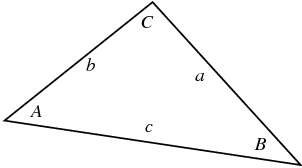
\includegraphics[width=20em]{cos1.png}

E�er, mesela C'nin 90 derece oldu�unu bilseydik, Pitagor kural�ndan

$$
c^2 = a^2 + b^2
$$

diyebilirdik. Ama $C < 90$ ise, farkl� bir form�l kullan�labilir,

$$
c^2 = a^2 + b^2 - 2 a b \cos C
$$

E�er $C=90$ ise $\cos(90) = 0$ oldu�u i�in Pitagor kural�n� elde etti�imizi
g�r�r�z. 

�stteki kurala Kosin�sler Kanunu denir, ispat� ��yle,

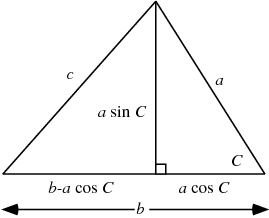
\includegraphics[width=20em]{cos2.png}

Ustteki ucgene bakarsak,

$$
c^2 = (a \sin C)^2 + (b-a\cos C)^2
$$

$$
a^2 \sin^2 C + b^2 - 2 a b \cos C + a^2 \cos^2 C
$$

$$
a^2 + b^2 - 2 a b \cos C
$$










Kaynaklar

[1] \url{https://mathworld.wolfram.com/LawofCosines.html}

[2] \url{https://tutorial.math.lamar.edu/classes/calcii/dotproduct.aspx}

[3] \url{http://sites.science.oregonstate.edu/math/home/programs/undergrad/CalculusQuestStudyGuides/vcalc/dotprod/dotprod.html}

[4] \url{https://mathinsight.org/dot_product}

\end{document}
